\documentclass[openany]{book}

\usepackage[utf8]{inputenc}
\usepackage[spanish]{babel}
\usepackage{hyperref}
\usepackage{graphicx}
\graphicspath{{img/}}
%\usepackage{mathrsfs}
%\usepackage{amsmath}
%\usepackage{amsthm}
%\usepackage{amssymb}
%\usepackage{amscd}
%\usepackage{amsfonts}
%\usepackage{bm}
\usepackage{url}
%\usepackage{moreverb}
\usepackage{fancyhdr}
%\usepackage{titling}
%\usepackage{titlesec}
%\usepackage{enumerate}
%\usepackage{listings}
%\usepackage{makeidx}
%\usepackage{multirow}
%\usepackage{array}
%\usepackage{pmat}
%\usepackage{algorithm}
%\usepackage{algpseudocode}
%\usepackage{rotating}
%\usepackage{braket}
%\usepackage{mathtools}
%\usepackage{slashbox}
%\usepackage{cancel}
%\usepackage{pst-all}
%\usepackage[stable]{footmisc}
%\usepackage{tikz}
%\usepackage{wallpaper} 
%\usepackage[style=super4colheaderborder,toc,acronym]{glossaries}
\usepackage[style=altlisthypergroup,toc,acronym]{glossaries}

\makeindex

\fancyhf{}
\fancyhead[LO]{\slshape \tiny \leftmark}
\fancyhead[RE]{\slshape \tiny \rightmark}
\fancyhead[RO,LE]{\scshape \thepage}
\renewcommand{\headrulewidth}{0.4pt}


\makeglossaries

\loadglsentries{glosario}
\loadglsentries{acronimos}



\begin{document}
\thispagestyle{empty}
\maketitle

\vspace{0.5cm}

\section{Resumen Ejecutivo}


\vspace{0.4cm}

\begin{keywords}
	Registro de imágenes, normalización.
\end{keywords}

\vspace{1cm}


\frontmatter
\pagestyle{fancy}
\newpage
~\vfill
\thispagestyle{empty}

\begin{table}[ht!]
	\centering
	\begin{tabular}{ccc}
		
\includegraphics[scale=.3]{chivo1} & 
\includegraphics[scale=.3]{chivo2} & 
\includegraphics[scale=.3]{chivo3}
	\end{tabular}
\end{table}
\noindent Copyright \copyright\ 2015 UTFSM UChile PUC UdeC USACH\\ % Copyright notice

\noindent \textsc{Publicado por UTFSM}\\ % Publisher

\noindent \textsc{chivo.cl}\\ % URL

\noindent Licensed under the Creative Commons Attribution-NonCommercial 3.0 Unported License (the ``License''). You may not use this file except in compliance with the License. You may obtain a copy of the License at \url{http://creativecommons.org/licenses/by-nc/3.0}. Unless required by applicable law or agreed to in writing, software distributed under the License is distributed on an \textsc{``as is'' basis, without warranties or conditions of any kind}, either express or implied. See the License for the specific language governing permissions and limitations under the License.\\ % License information

\noindent \textit{Primera impresión, Abril 2015} % Printing/edition date


\chapter*{Agradecimientos}
\addcontentsline{toc}{chapter}{Agradecimientos}

Dedicatoria\ldots

\renewcommand{\listfigurename}{Índice de imágenes}
\renewcommand{\listtablename}{Índice de tablas}
\renewcommand{\figurename}{Imagen}
\renewcommand{\tablename}{Tabla}
\tableofcontents
\addcontentsline{toc}{chapter}{Índice general}
\listoftables
\addcontentsline{toc}{chapter}{Índice de tablas}
\listoffigures
\addcontentsline{toc}{chapter}{Índice de imágenes}
\addcontentsline{toc}{chapter}{Prefacio}
\chapter*{Prefacio}

Palabras previas\ldots

\addcontentsline{toc}{chapter}{Colaboradores}
\chapter*{Colaboradores}

La lista de colaboradores\ldots

\chapter*{Introducción}
\addcontentsline{toc}{chapter}{Introducción}

Este libro tiene por objetivo\ldots


\mainmatter
\part{Observatorio virtual}
Desde el año 2002, proyectos de Observatorios Virtuales (VO’s, por sus siglas en ingl\'es) comenzaron a integrar la Alianza Internacional de Observatorios Virtuales bajo el \emph{Guidelines for Participation}\footnotemark{}.

\footnotetext{La documentación se puede encontrar en \url{http://www.ivoa.net/documents/latest/IVOAParticipation.html}.}

Esos proyectos fueron fundados bajo programas privados y gubernamentales nacionales e internacionales en colaboración con centros de estudios científicos, universidades y otros. Quienes integran este proyecto, el Observatorio Virtual, comparten conocimientos entre ellos y la comunidad de modo estandarizado, siendo ellos mismos quienes desarrollan estos estándares para el intercambio de información e interoperabilidad.

La Tab.~\ref{tab:memivoa} muestra los miembros de IVOA hasta abril de 2015\footnotemark.

\footnotetext{\url{http://www.ivoa.net/about/member-organizations.html}.}

\begin{table}[ht!]
	\centering
	\begin{tabular}{c|p{2.3in}|p{2.5in}}
		Proyecto & Nombre & Dirección \\\hline\hline
		NOVA & Nuevo Observatorio Virtual Argentino & \url{http://nova.conicet.gov.ar/} \\\hline
		ArVO & Armenian Virtual Observatory & \url{http://www.aras.am/Arvo/arvo.htm} \\\hline
		AstroGrid & UK's Virtual Observatory & \url{http://www.astrogrid.org/} \\\hline
		Aus-VO & Australian Virtual Observatory & \url{http://aus-vo.org.au/} \\\hline
		BRAVO & Brazilian Virtual Observatory & \url{http://bravo.iag.usp.br/} \\\hline
		CVO & Canadian Virtual Observatory & \url{http://www.cadc-ccda.hia-iha.nrc-cnrc.gc.ca/cvo/} \\\hline
		ChiVO & Chilean Virtual Observatory & \url{http://www.chivo.cl/} \\\hline
		China-VO & Chinese Virtual Observatory & \url{http://www.china-vo.org/} \\\hline
		ESA-VO & European Space Agency Virtual Observatory & \url{http://www.sciops.esa.int/index.php?project=SAT\&page=ESAVOIntro} \\\hline
		EURO-VO & European Virtual Observatory & \url{http://www.euro-vo.org/} \\\hline
		GAVO & German Astrophysical Virtual Observatory & \url{http://www.g-vo.org/} \\\hline
		HVO & Hungarian Virtual Observatory & \url{http://hvo.elte.hu/en/} \\\hline
		JVO & Japanese Virtual Observatory & \url{http://jvo.nao.ac.jp/} \\\hline
		OV-France & Observatoires Virtuels France & \url{http://www.france-vo.org/} \\\hline
		RVO & Russian Virtual Observatory & \url{http://www.inasan.rssi.ru/eng/rvo/} \\\hline
		SA\textsuperscript{3} & South African Astroinformatics Alliance & \url{http://www.sa3.ac.za/} \\\hline
		SVO & Spanish Virtual Observatory & \url{http://svo.cab.inta-csic.es/main/index.php} \\\hline
		VObs.it & Italian Virtual Observatory & \url{http://vobs.astro.it/} \\\hline
		UKR VO & Ukrainian Virtual Observatory & \url{http://www.ukr-vo.org/} \\\hline
		VAO & US Virtual Astronomical Observatory & \url{http://www.usvao.org/} \\\hline
		VO-I & Virtual Observatory India & \url{http://vo.iucaa.ernet.in/~voi/} \\
	\end{tabular}
	\caption{Integrantes de IVOA.}
	\label{tab:memivoa}
\end{table}

Con la incorporación de ChiVO a la lista de organizaciones miembro de IVOA, el continente americano se equipara en cantidad de VO's al continente asiático\footnotemark{}, siendo el europeo el que mantiene el liderato. La incorporación de Chile a este selecto grupo no hace más que consolidar la postura a nivel informático del país con mayor presencia de observatorios astronómicos a nivel mundial.

\footnotetext{Esto es considerando a Armenia y Rusia como miembros asiáticos. Si se les considera como europeos, Am\'erica es el segundo continente con mayor cantidad de VO's.}

Considerando todo lo anterior, al comienzo del proyecto se detalló un listado de requerimientos, los cuales se repasan a continuación:

\begin{description}
	\item[Buscar por coordenadas o región en el cielo] Se podrá realizar búsquedas de posición mediante coordenadas y radio angular (cónicas) o por	región del cielo. Los parámetros de las coordenadas pueden ser en distintos sistemas como ecuatorial, eclíptico, galáctico o supergaláctico. Los parámetros ingresados se convertirán al sistema de la fuente de datos, para así poder realizar las búsquedas, IVOA utiliza los sistemas de coordenadas ICRS y ecuatoriales J2000. En un principio, el sistema ofrecerá servicio de búsqueda por coordenadas cónicas y más adelante, en caso de ser vía un portal web, se ofrecerá búsqueda por región del cielo. El sistema tambi\'en deberá permitir buscar simultáneamente un listado de coordenadas.
	\item[Buscar por nombre o tipo de objeto] El sistema deberá permitir buscar por nombres de objetos que se encuentren definidos en Sesame, del \emph{Centre de Donn\'ees astronomiques de Strasbourg} (CDS). Por otro lado, la búsqueda por tipo o subtipo de objeto, tales como estrellas en formación, estrellas nebulosas planetarias, supernovas, galaxias, cometas, entre otros, permitirá al usuario encontrar datos relacionados con una problemática en especial. En un principio, el sistema realizará estas búsquedas acorde a la información presente en los catálogos. A futuro, el sistema deberá permitir minería de datos para detección de tipos de objetos similares, esto es posible debido a que existen clasificaciones discretas que permiten clasificar los objetos que se encuentran en las observaciones. Este tipo de búsquedas, se transforman en búsquedas por coordenadas, ya que al buscar por un nombre, por ejemplo, Sesame responde con la correspondiente ubicación del objeto en coordenadas. Y luego de ello se procede a realizar la búsqueda por coordenadas correspondiente. El resultado de la búsqueda deberá facilitar la obtención de datos para ser analizados como secuencias de tiempo.
	\item[Buscar por metadatos espectrales] Se podrá realizar búsquedas por metadatos espectrales, lo cual consiste en búsqueda por banda o	rango de frecuencia, búsquedas por líneas espectrales y corrimiento al rojo o búsquedas por resolución espectral. Específicamente, hay dos enfoques:
		\begin{itemize}
			\item Galáctico: Por frecuencia en reposo y velocidad radial.
			\item Extragaláctico: Por frecuencia en reposo y corrimiento al rojo.
		\end{itemize}
		La frecuencia en reposo incluye búsquedas por mol\'ecula, transición de mol\'ecula (vibracional, rotacional o electrónica) o frecuencia de línea espectral.
	\item[Buscar por metadatos espaciales] Se podrá realizar búsquedas espaciales en base a parámetros relacionados con rangos de resolución angular y campos de visión y siempre en base a coordenadas. Los parámetros de las coordenadas pueden ser en distintos sistemas como ecuatorial, eclíptico, galáctico o supergaláctico. Los parámetros ingresados se convertirán al sistema de la fuente de datos, para así poder realizar las búsquedas. Además, se podrá especificar parámetros relacionados con la forma de las observaciones (rectangulares o redondas).
	\item[Buscar por metadatos temporales] Se podrá realizar búsquedas por metadatos temporales que pueden ser clasificadas en dos tipos de	búsquedas:
		\begin{itemize}
			\item Cuando fue realizada la observación, incluyendo cuantas veces se observó un objeto y/o el	intervalo entre observaciones.
			\item Nivel de ruido, duración de la observación o tiempo de integración. Dado un ruido, se necesita un tiempo de integración que depende de la frecuencia observada y del clima.
		\end{itemize}
	\item[Buscar por polarización] Cada imagen se puede dividir en cuatro parámetros llamados los parámetros de Stokes o en dos: izquierda y derecha. En radio astronomía no suele hacerse debido a que requiere una alta precisión	del instrumento, en el caso de ALMA se requiere que est\'e lista la calibración. El sistema debe permitir buscar si existe o no polarización en alguno de los parámetros de Stokes: I, Q, U o V.
	\item[Cruzamiento de información] La búsqueda cruzada debe permitir al usuario realizar las búsquedas mencionadas anteriormente	en múltiples fuentes de datos distribuidos globalmente, sin importar su tipo. Lo que permitirá obtener todos los datos existentes sobre un objeto o área espacial y así evitar realizar observaciones innecesarias debido al descubrimiento de observaciones existentes. Los tipos de fuentes pueden ser Sesame, ALMA u Observatorios Virtuales, que cumplan con los estándares de IVOA. La búsqueda de un mismo objeto en distintas fuentes de información, debido a que en cada fuente el instrumento tiene un margen de error en cuanto a la posición del objeto, debe ser capaz de realizar	una intersección entre los radios de margen de error de las distintas fuentes para identificar al objeto en una búsqueda cruzada.
	\item[Simulaciones] Es a veces necesario realizar comparaciones con observaciones obtenidas a trav\'es de simulaciones,	así cómo es costoso realizar una observación dos veces, para una simulación puede ser aún más, debido a que dependiendo de la magnitud, hay simulaciones que requieren una gran capacidad de cómputo.
	\item[Servicios Bibliográficos] Las herramientas existentes cumplen su función correctamente. Por ello, basta con que al buscar un objeto, se despliegue tambi\'en resultados de investigaciones que se hayan realizado al respecto con	un enlace a SIMBAD o similares.
\end{description}



\chapter{Capa de usuario}

Inicialmente, el sistema en su forma gráfica fue pensado sólo como una interfaz de dos partes: una básica (Img.~\ref{img:basicQuery}) y una avanzada (Img.~\ref{img:advancedQuery}), lo cual fue con tiempo evolucionando.

\begin{figure}[ht!]
	\centering
	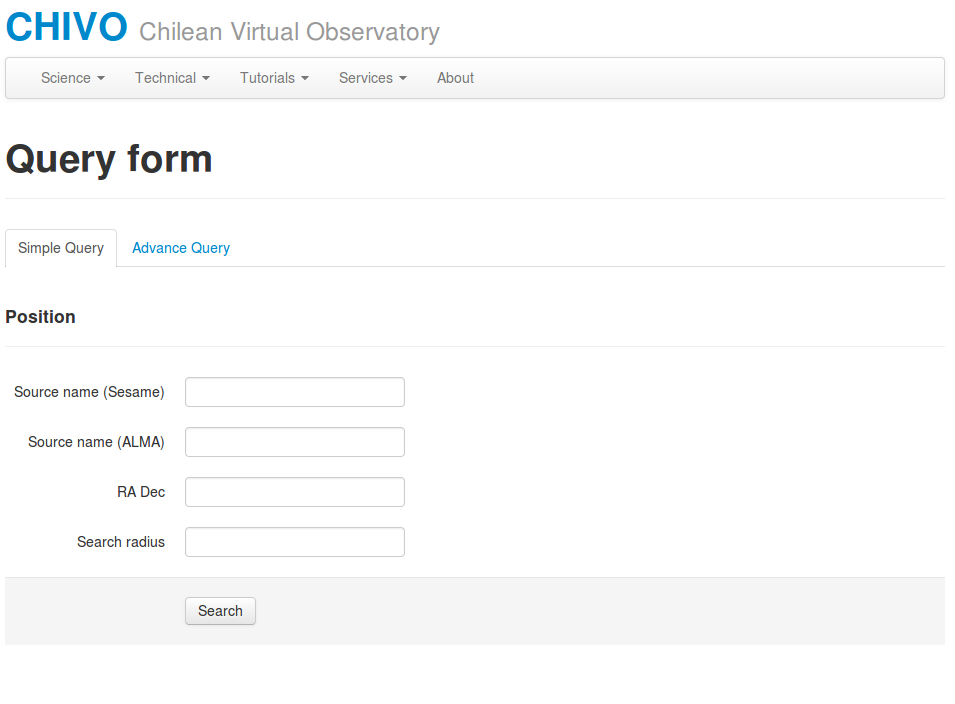
\includegraphics[scale=.4]{basicQuery}
	\caption{Maqueta inicial para búsqueda básica.}
	\label{img:basicQuery}
\end{figure}

\begin{figure}[ht!]
	\centering
	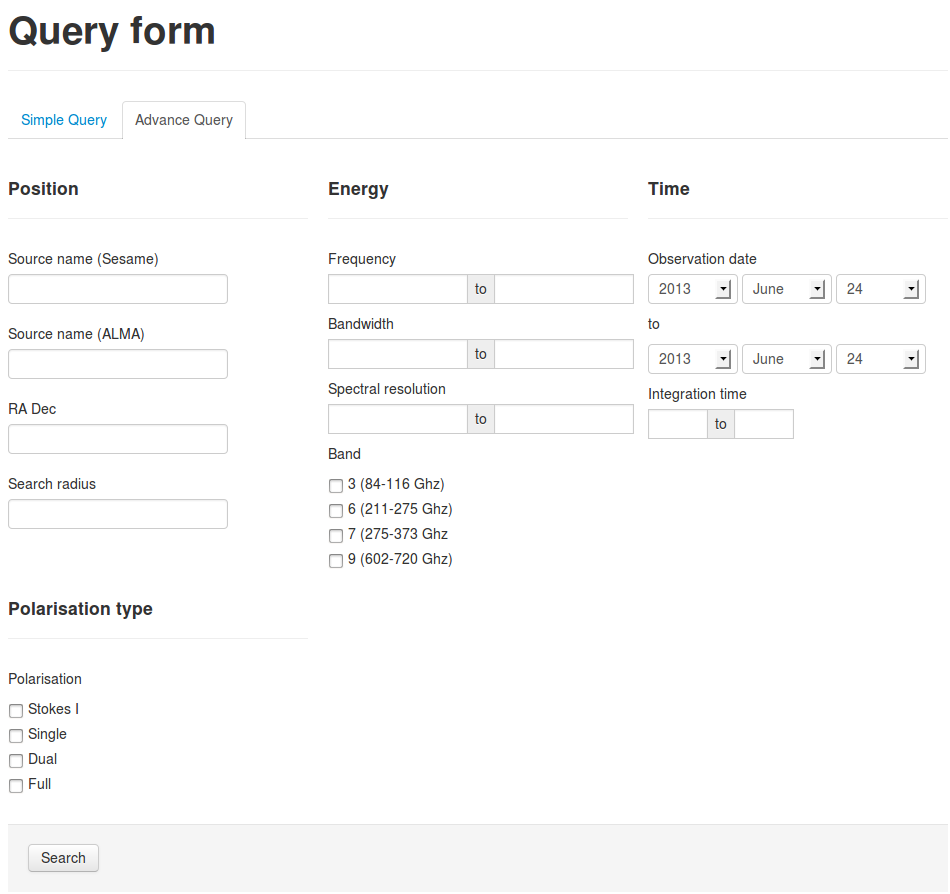
\includegraphics[scale=.4]{advancedQuery}
	\caption{Maqueta inicial para búsqueda avanzada.}
	\label{img:advancedQuery}
\end{figure}

\chapter{Capa de apliación}

La capa de aplicación, o \emph{endpoint}\ldots

\chapter{Capa de datos}

La capa de datos, o \emph{backend}\ldots

\chapter{Pruebas de integración}

En las pruebas de integración \cite{cloud}\ldots


\part{M\'etodos de búsqueda semántica}
Los m\'etodos de búsqueda semántica\ldots


\part{M\'etodos de minería de datos}
Los m\'etodos de minería de datos\ldots


\part{Anexos}
\appendix
\chapter{Arquitectura IVOA}

El \gls{vo} es un framework que ayuda a resolver distintos problemas que enfrenta la comunidad astronómica internacional. Uno de los problemas está relacionado al acceso a los datos, por lo que en IVOA diseñaron tecnologías y estándares formalmente definidos, que permitan el acceso unificado y transparente a distintos servidores con datos astronómicos.

El beneficio que conlleva es considerable, ya que estos estándares, protocolos, tecnologías y arquitectura, ayudan a la comunidad al proceso de creación de servicios, portales web, aplicaciones de escritorio, etc. Todo visto del punto de vista de ingeniería de software.

\section{Arquitectura VO por nivel}

\gls{ivoa} dentro de sus documentos presenta distintos niveles de arquitectura \cite{ivoaArq}, con el objetivo de ir aclarando incrementalmente las funcionalidades (basadas en necesidades) que requiere un VO.

\subsection{Arquitectura Nivel 0}

La arquitectura más básica que aclara el concepto de VO, se compone de 3 capas (Img.~\ref{img:arq0}):

\begin{figure}[ht!]
	\centering
	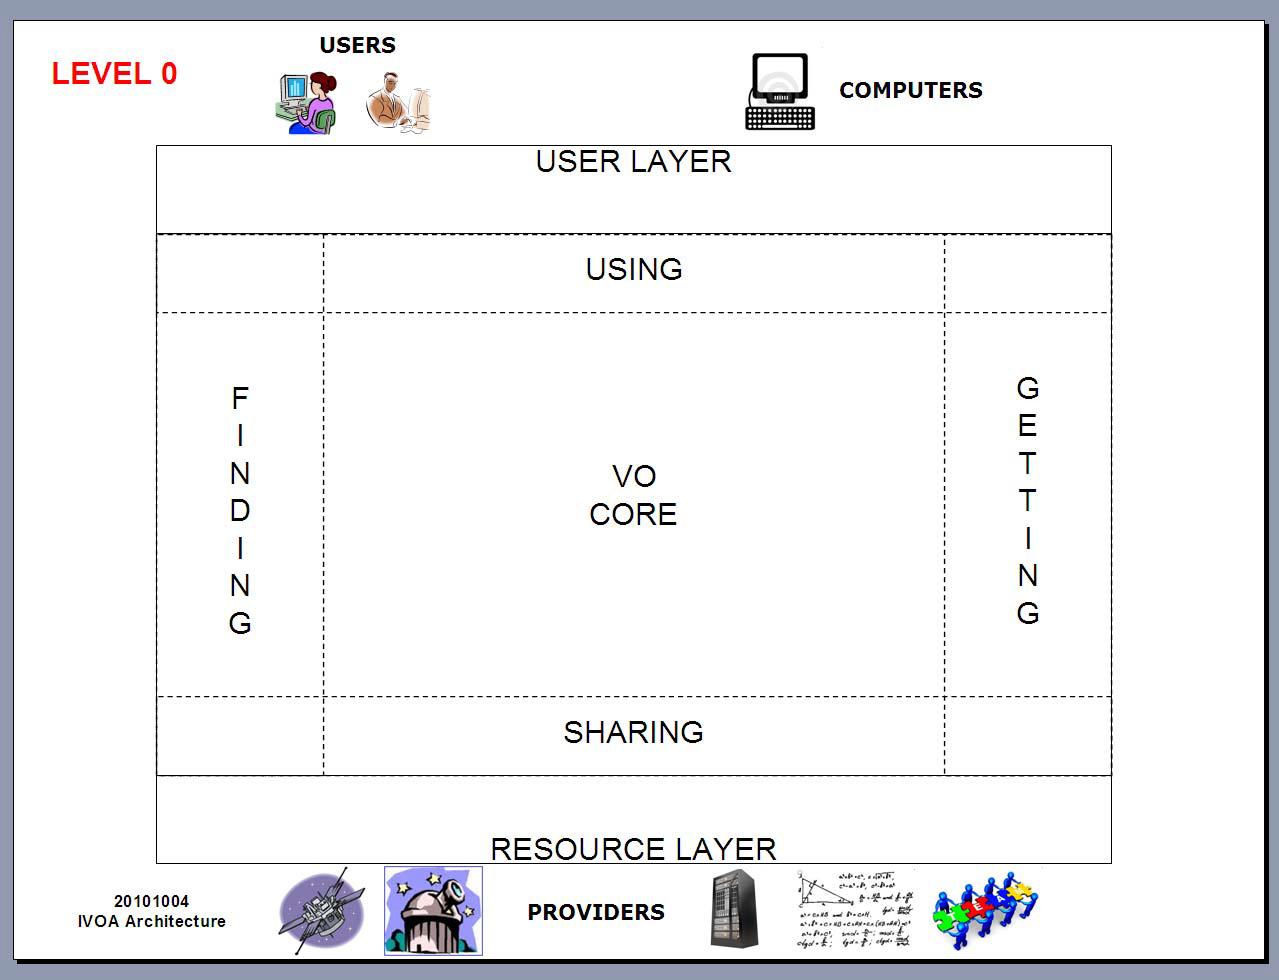
\includegraphics[scale=.2]{arq0}
	\caption{Arquitectura nivel 0.}
	\label{img:arq0}
\end{figure}

\begin{enumerate}
	\item Capa de recursos: compilado de datos astronómicos provenientes de distintos instrumentos.
	\item Capa de usuarios: investigadores que buscan consumir datos.
	\item Capa intermedia: es la capa que permite conectar las dos capas anteriores de manera transparente para los investigadores. Esta interacción se puede llevar a cabo buscando u obteniendo datos.
\end{enumerate}

\subsection{Arquitectura Nivel 1}

La arquitectura nivel 1 mantiene la misma cantidad de capas pero se especifica aún más (Img.~\ref{img:arq1}):

\begin{figure}[ht!]
	\centering
	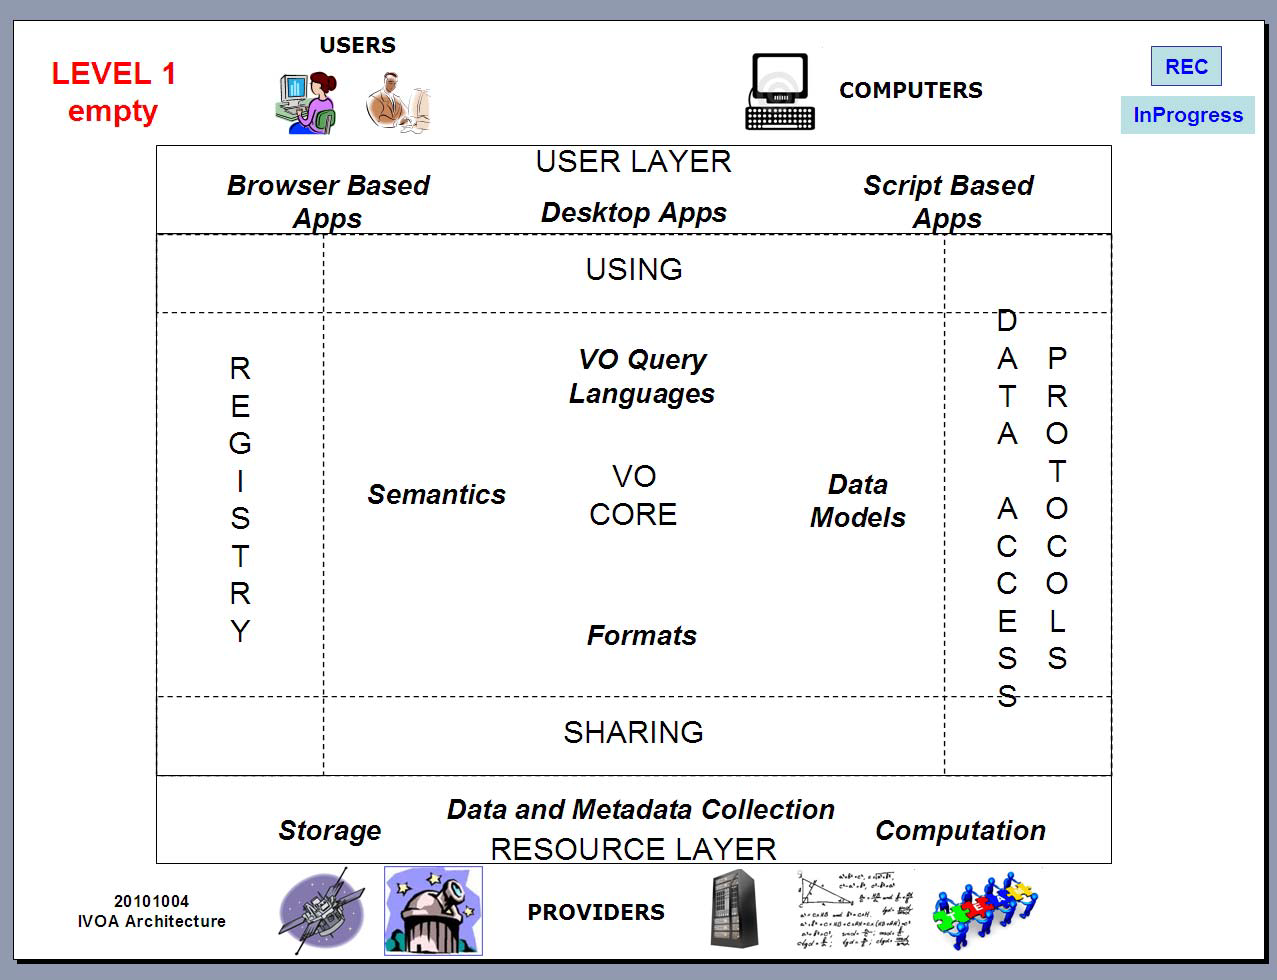
\includegraphics[scale=.2]{arq1}
	\caption{Arquitectura nivel 1.}
	\label{img:arq1}

\end{figure}

\begin{enumerate}
	\item Capa de recursos: está compuesto de una colección de datos y provenientes de distintos servidores.
	\item Capa de usuarios: un consumidor puede querer acceder a los datos desde un navegador, escritorio, o mediante un script.
	\item Capa intermedia: crea un framework para compartir los datos, compuesto por \gls{voql}, \emph{Data Models}, \emph{semantics}, \emph{Formats}.
\end{enumerate}

\subsection{
Arquitectura Nivel 2}

La arquitectura nivel 2 es lo que se entiende por un VO regido por estándares y protocolos de IVOA. La idea de esta figura es seccionar cada estándar relacionándolo específicamente a la capa a la cual pertenece (Img.~\ref{img:arq2}).


\begin{figure}[ht!]
	\centering
	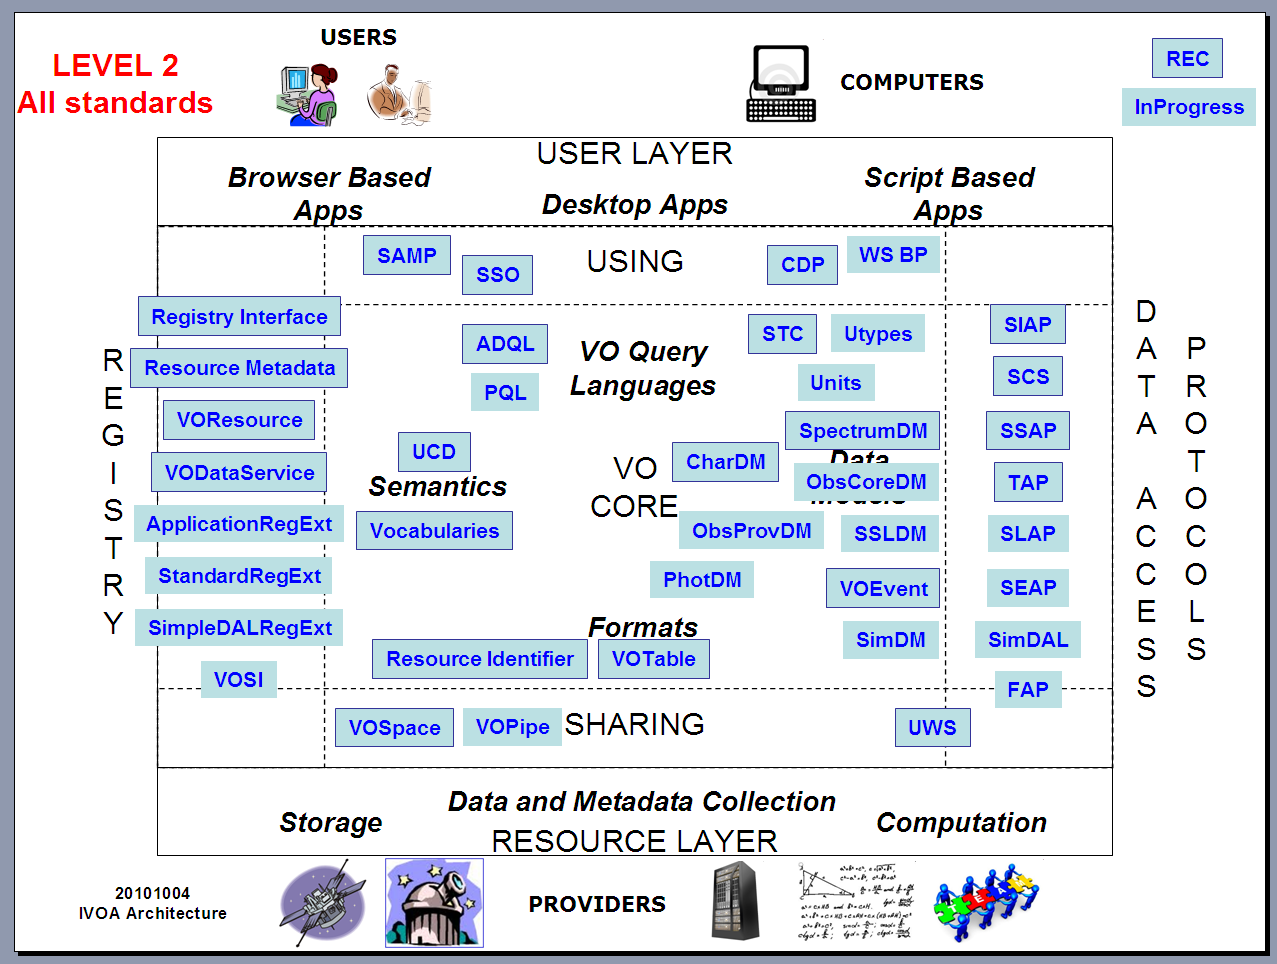
\includegraphics[scale=.2]{arq2}
	\caption{Arquitectura nivel 2.}
	\label{img:arq2}
\end{figure}


\backmatter
\clearpage
	
\glsaddall
\printglossary[title=Lista de términos]
\printglossary[type=\acronymtype,title=Lista de acrónimos]
\newpage	


\thispagestyle{empty}
\addcontentsline{toc}{section}{Bibliografía}
\bibliographystyle{plain}
\bibliography{bibliografia}




\end{document}
